\section{TX}
\label{sec:tx}
\textit{\hyperlink{schematic.5}{schematic}}

\subsection{ADF4158 Frequency Synthesizer}
\label{sec:adf4158-freq-synth}

\subsubsection{Overview}
\label{sec:adf4158-overview}

The \href{http://www.analog.com/media/en/technical-documentation/data-sheets/ADF4158.pdf}{ADF4158}
is a 6.1GHz fractional-n frequency synthesizer. A block diagram describing its functionality is shown in
Figure~\ref{fig:adf4158-block-diagram}.

\begin{figure}[h]
        \centering
        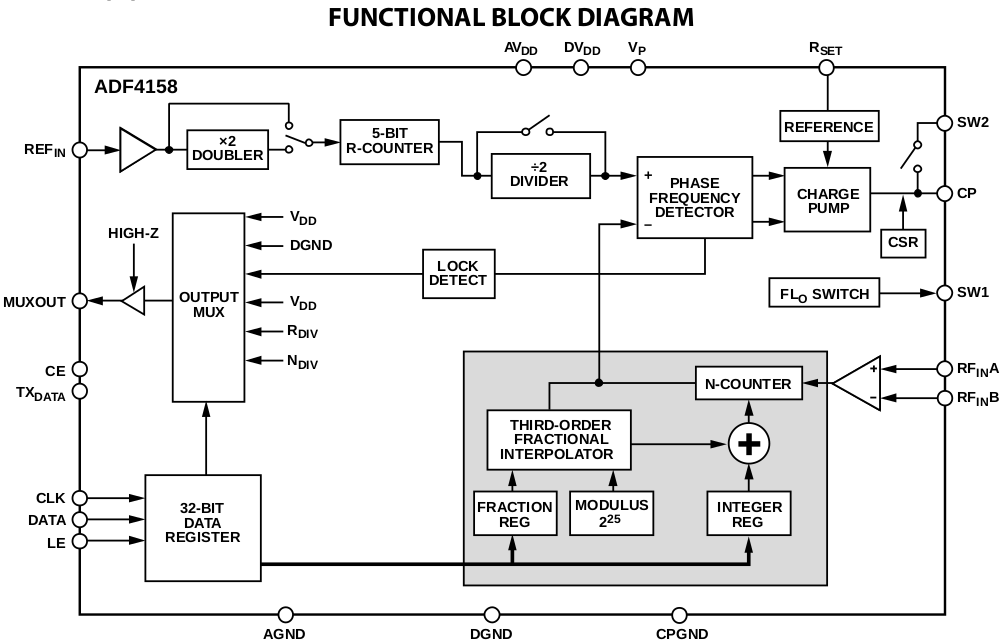
\includegraphics[width=0.75\textwidth]{data/adf4158-block-diagram.png}
        \caption{ADF4158 block diagram.}
        \label{fig:adf4158-block-diagram}
\end{figure}

The ADF4158 relies on an external VCO, described in \cref{sec:hmc431lp4rf}, whose output frequency
is given by Equation~\ref{eq:adf4158-rfout}. The output resolution is
$f_{\text{RES}} = f_{\text{PFD}}/2^{25}$ (see Equation~\ref{eq:adf4158-rfout} and its corresponding
parameter table for an explanation of $f_{\text{PFD}}$). The $2^{25}$ arises from the FRAC value
(set in registers 0 and 1) which is given 25 bits.

\begin{align}
  \text{RF}_{\text{OUT}} &= f_{\text{PFD}} \times \left(\text{INT} +
                           \left(\text{FRAC}/2^{25}\right)\right) \label{eq:adf4158-rfout} \\
  f_{\text{PFD}} &= \text{REF}_{\text{IN}} \times \left[\left(1 + D\right)/\left(R\times \left(1 +
                   T\right)\right) \right] \nonumber
\end{align}

\label{tab:adf4158-rfout-equation-vars}
\begin{tabularx}{\textwidth}{l X>{\raggedright\arraybackslash}X}
        \toprule
        \textbf{Parameter/Variable} & \textbf{Description} \\
        \midrule
        \endhead{}

        $\text{RF}_{\text{OUT}}$ & The VCO's output frequency. This is the frequency that's amplified for
        transmission. \\
        $f_{\text{PFD}}$ & The input frequency to the PFD post prescaling. In our case this is 20MHz. \\
        INT & The N counter that has a multiplicative effect on the VCO output frequency. \\
        FRAC & FRAC is the numerator of the fractional number added to INT. This is what distinguishes
        fractional-n synthesis from integer-n synthesis. It allows greater precision for the VCO
        output frequency without significantly increasing the prescalers and N counter. \\
        $\text{REF}_{\text{IN}} $ & The reference input frequency, which in our case is a 40MHz clock
        signal from the fanout buffer on the top level of the schematic. \\
        D & The doubler bit, which can be 0 or 1. If set to 1, the $\text{REF}_{\text{IN}}$ frequency is
        doubled before arriving at the R counter. \\
        R & The input prescaler. \\
        T & The divide- by-2 bit, which can be 0 or 1 and divides the frequency by 2 between the R
        prescaler and PFD. \\

        \bottomrule
\end{tabularx}

\subsubsection{Waveform Generation}
\label{sec:adf4158-waveform-generation}

The ADF4158 is capable of producing several different waveforms. The one used in this design is a
sawtooth ramp in frequency as a function of time, shown in
Figure~\ref{fig:adf4158-sawtooth-ramp}. There are 3 different parameters that determine the shape of
a ramp: (1) frequency deviation (the amount the frequency increases at each time step), (2) timeout
interval (the amount of time between each time step) and (3) the number of time steps. This is shown
diagrammatically in Figure~\ref{fig:adf4158-waveform-timing}. The equations governing these
parameters are given in Equation~\ref{eq:adf4158-waveform}. The number of steps is set directly in
register 6. In our configuration $f_{\text{DEV}} = 300\si{kHz}$ and $\text{Timer} = 0.5\si{\mu s}$,
which given that the number of steps is equal to 2000 and the starting frequency is 5.3GHz, the
sawtooth will ramp from 5.3GHz to 5.9GHz in 1ms. We also use a delay between bursts of
2ms. Equation~\ref{eq:adf4158-delay} is used to derive this.

\begin{align}
  f_{\text{DEV}} &= \left(f_{\text{PFD}}/2^{25}\right) \times \left(\text{DEV}\times
                   2^{\text{DEV\_OFFSET}}\right) \label{eq:adf4158-waveform} \\
  \text{Timer} &= \text{CLK}_1 \times \text{CLK}_2 \times \left(1/f_{\text{PFD}}\right) \nonumber
\end{align}

\label{tab:adf4158-waveform-equation-vars}
\begin{tabularx}{\textwidth}{l X>{\raggedright\arraybackslash}X}
        \toprule
        \textbf{Parameter/Variable} & \textbf{Description} \\
        \midrule

        \endhead

        $f_{\text{DEV}}$ & The frequency deviation for each frequency jump during ramp. \\
        $f_{\text{PFD}}$ & The input frequency to the PFD post prescaling. In our case this is 20MHz. \\
        DEV & A 16-bit value set in register 5. \\
        DEV\_OFFSET & A 4-bit word set in register 5. \\
        Timer & The time between each frequency hop. \\
        CLK\textsubscript{1} & A 12-bit clock divider set in register 2. \\
        CLK\textsubscript{2} & Another 12-bit clock divider set in register 4. \\

        \bottomrule
\end{tabularx}

\begin{equation}
        \label{eq:adf4158-delay}
        \text{Delay} = t_{\text{PFD}} \times \text{CLK}_1 \times \text{Delay Start Word}
\end{equation}

\label{tab:adf4158-delay-equation-vars}
\begin{tabularx}{\textwidth}{l X>{\raggedright\arraybackslash}X}
        \toprule
        \textbf{Parameter/Variable} & \textbf{Description} \\
        \midrule

        \endhead

        Delay & The delay between bursts. This is shown graphically in Figure~\ref{fig:adf4158-delay}. \\
        $f_{\text{PFD}}$ & The input frequency to the PFD post prescaling. In our case this is 20MHz. \\
        CLK\textsubscript{1} & A 12-bit clock divider set in register 2. \\
        Delay Start Word & A 12-bit value set in register 7. \\

        \bottomrule
\end{tabularx}

\begin{figure}[h]
        \centering
        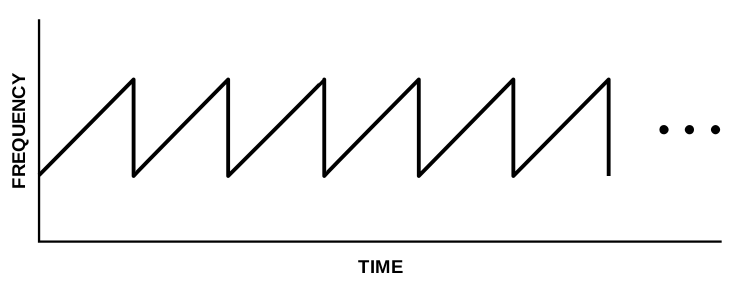
\includegraphics[width=0.5\textwidth]{data/adf4158-sawtooth-ramp.png}
        \caption{Sawtooth ramp.}
        \label{fig:adf4158-sawtooth-ramp}\end{figure}

\begin{figure}[h]
        \centering
        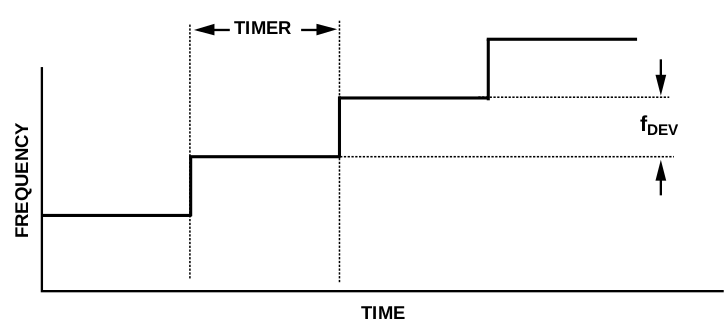
\includegraphics[width=0.5\textwidth]{data/adf4158-waveform-timing.png}
        \caption{Waveform timing.}
        \label{fig:adf4158-waveform-timing}
\end{figure}

\begin{figure}[h]
        \centering
        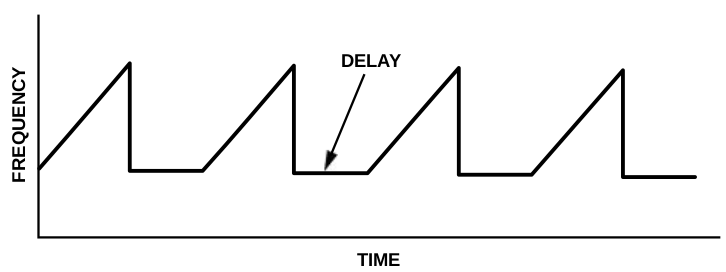
\includegraphics[width=0.5\textwidth]{data/adf4158-delay.png}
        \caption{Delay between ramps for sawtooth mode.}
        \label{fig:adf4158-delay}
\end{figure}

\subsubsection{Configuration Registers}
\label{sec:adf4158-config-regs}

The ADF4158 contains 8 configuration registers. The configurations are shown in the tables
below. All reserved bits should be set to 0. The control bits are the least significant 3 bits of
each register and are set to the register number for each register (e.g. register 0 is 000 and
register 1 is 001). I've left these out of the tables because their values are obvious.

\label{tab:adf4158-reg-map-0}
\begin{tabularx}{\textwidth}{l l l X>{\raggedright\arraybackslash}X}
        \caption{FRAC/INT REGISTER (R0) MAP} \\
        \toprule
        \textbf{Bits} & \textbf{Mnemonic} & \textbf{Value} & \textbf{DESCRIPTION} \\
        \midrule

        \endhead{}

        3--14 & FRAC(MSB) & 0 & This sets the 12 most significant bits of FRAC. We leave the fractional
        value at 0. \\
        15--26 & INT & 265 & This is the feedback, or N, counter. \\
        27--30 & MUXOUT Control & 15 & This enables ``readback to muxout'' which allows interrupting
        waveform generation and reading back the frequency at the time of
        interrupt. The functionality is not fully setup on the board(muxout
        connects to a DNP NMOS) and TX\_DATA, which can trigger the
        interrupt, is set to 0 by the FPGA HDL and left there. \\
        31 & Ramp On & 1 & This bit enables the ramp. \\

        \bottomrule
\end{tabularx}

\label{tab:adf4158-reg-map-1}
\begin{tabularx}{\textwidth}{l l l X>{\raggedright\arraybackslash}X}
        \caption{LSB FRAC REGISTER(R1) MAP} \\
        \toprule
        \textbf{Bits} & \textbf{Mnemonic} & \textbf{Value} & \textbf{DESCRIPTION} \\
        \midrule

        \endhead

        3-14 & Reserved & 0 & All reserved bits set to 0. \\
        15-27 & FRAC(LSB) & 0 & This sets the 13 least significant bits of FRAC. We leave the fractional
        value at 0. \\
        28-31 & Reserved & 0 & All reserved bits set to 0. \\

        \bottomrule
\end{tabularx}

\label{tab:adf4158-reg-map-2}
\begin{tabularx}{\textwidth}{l l l X>{\raggedright\arraybackslash}X}
        \caption{R-DIVIDER REGISTER(R2) MAP} \\
        \toprule
        \textbf{Bits} & \textbf{Mnemonic} & \textbf{Value} & \textbf{DESCRIPTION} \\
        \midrule

        \endhead

        3--14 & CLK\textsubscript{1} Divider & 10 & One of the determinants of the duration of a timestep in
        waveform generation. See
        \cref{sec:adf4158-waveform-generation} for more
        details. \\
        15--19 & R-Counter & 1 & This 5-bit segment is used to divide the frequency of the reference signal
        before it enters the PFD. We leave it at 1 and thus do not use it to
        divide the frequency. \\
        20 & Reference Doubler & 0 & We leave this at 0 and thus do not use the doubler to double the
        reference signal frequency before input to the PFD. The maximum input
        frequency for the PFD is 30MHz and so doubling our 20MHz signal (we
        used the divider to divide the 40MHz signal by 2) would violate this
        condition. \\
        21 & RDIV2 & 1 & Inserts a divide-by-2 toggle flip-flop between the R-counter and PFD. This
        provides a 50\% duty cycle that allows cycle slip reduction to be used which
        improves lock times. \\
        22 & Prescaler & 1 & The prescaler limits the INT value and through that the maximum frequency to
        3GHz. Since we have an INT value of 265 and our maximum frequency is almost
        double 3GHz we set this to 1. \\
        23 & Reserved & 0 & All reserved bits set to 0. \\
        24--27 & Charge Pump Current Setting & 0 & Sets the current to the minimum value which is 0.31mA
        and is the level necessary to use cycle slip reduction
        which we are. \\
        28 & CSR Enable & 1 & Enables cycle slip reduction which provides better lock times. \\
        29--31 & Reserved & 0 & All reserved bits are set to 0. \\

        \bottomrule
\end{tabularx}

\label{tab:adf4158-reg-map-3}
\begin{tabularx}{\textwidth}{l l l X>{\raggedright\arraybackslash}X}
        \caption{FUNCTION REGISTER(R3) MAP} \\
        \toprule
        \textbf{Bits} & \textbf{Mnemonic} & \textbf{Value} & \textbf{DESCRIPTION} \\
        \midrule

        \endhead{}

        3 & Counter Reset & 0 & When this is set to 1, the synthesizer counters are held in reset. For
        normal operation we set this to 0. \\
        4 & Charge Pump Three-State & 0 & Holds the charge pump in three-state mode if set to 1. For
        normal operation it must be set to 0. \\
        5 & Power-Down & 0 & Setting this to 1 powers down the device. Setting it to 0 allows normal
        operation. \\
        6 & PD Polarity & 1 & Set to 1 for positive VCO characteristics. Set to 0 for negative VCO
        characteristics. Since our VCO outputs a positive voltage signal we set this
        to 1. \\
        7 & LDP & 0 & Sets the minimum number of PFD cycles before a lock detect can be set. \\
        8 & FSK Enable & 0 & Disables FSK modulation. \\
        9 & PSK Enable & 0 & Disables PSK modulation. \\
        10-11 & Ramp Mode & 0 & Sets the waveform as a continuous sawtooth. \\
        12-13 & Reserved & 0 & All reserve bits are set to 0. \\
        14 & SD Reset & 0 & Setting this to 0 resets the $\Sigma-\Delta$ modulator on each write to
        register 0, which is the recommended operation. Setting this to 1 disables
        resetting the modulator. \\
        15 & N SEL & 0 & When set to 1, this creates an additional delay in setting INT and FRAC which can
        prevent the PLL overshooting. Since we set INT once and do not update it, this is
        not necessary and we leave it as 0. \\
        16-31 & Reserved & 0 & All reserve bits are set to 0. \\

        \bottomrule
\end{tabularx}

\label{tab:adf4158-reg-map-4}
\begin{tabularx}{\textwidth}{l l l X>{\raggedright\arraybackslash}X}
        \caption{TEST REGISTER(R4) MAP} \\
        \toprule
        \textbf{Bits} & \textbf{Mnemonic} & \textbf{Value} & \textbf{DESCRIPTION} \\
        \midrule

        \endhead{}

        3--6 & Reserved & 0 & All reserved bits are set to 0. \\
        7-18 & CLK\textsubscript{2} Divider & 1 & This is used to set the timeout interval in ramp
        generation. See
        \cref{sec:adf4158-waveform-generation}for more
        information. \\
        19-20 & CLK DIV Mode & 3 & This enables ramp divider mode, which specifies that
        CLK\textsubscript{1} and CLK\textsubscript{2} are used for ramp
        generation. \\
        21-22 & Readback to MUXOUT & 3 & Confusingly, this has been set to 3, which corresponds to neither
        of the supported values. Since we don't actually use the MUXOUT, this seems to be fine. If, at
        some point in the future, we do use the MUXOUT we will probably
        need to fix this. \\
        23-24 & Negative Bleed Current & 0 & This setting can help improve performance in the dead
        zone. We've disabled it. Note that this setting and readback
        to MUXOUT cannot simultaneously be enabled. To understand
        this setting better refer to \href{http://www.analog.com/media/en/technical-documentation/application-notes/AN-1154.pdf?doc=ADF4158.pdf}{AN-1154
          Application Note}. \\
        25 & Reserved & 0 & All reserved bits are set to 0. \\
        26-30 & $\Sigma-\Delta$ modulator mode & 0 & 0 enables this during normal operation. We can set it
        to 14 when FRAC=0. Even though we've set FRAC to 0,
        we have left this as 0 which seems strange. It
        shouldn't cause anything to malfunction, but may
        cause the ADF4158 to draw more power. We should
        experiment with setting this to 14 when using the
        actual board. \\
        31 & LE SEL & 0 & LE is the load enable pin which we use to load data onto the ADF4158's internal
        registers. Setting this to 0 enables the default operation of using the pin to
        set LE. Setting it to 1 would synchronize it with the reference signal. \\

        \bottomrule
\end{tabularx}

\label{tab:adf4158-reg-map-5}
\begin{tabularx}{\textwidth}{l l l X>{\raggedright\arraybackslash}X}
        \caption{DEVIATION REGISTER (R5) MAP} \\
        \toprule
        \textbf{Bits} & \textbf{Mnemonic} & \textbf{Value} & \textbf{DESCRIPTION} \\
        \midrule

        \endhead{}

        3--18 & Deviation Word & 31457 & This is used to set the size of successive frequency jumps during
        ramp. See \cref{sec:adf4158-waveform-generation} for more
        information. \\
        19--22 & Deviation Offset Word & 4 & This is also used to set the size of successive frequency
        jumps during ramp. See \cref{sec:adf4158-waveform-generation}
        for more information. \\
        23 & Deviation Select & 0 & Setting this bit to 1 is used for FSK as described on page 28 of the
        datasheet. Since we do not use FSK we leave this as 0. \\
        24 & Ramp 2 Enable & 0 & Setting this bit to 1 allows a second ramp with different settings than
        the first. We only need the first ramp. \\
        25 & FSK Ramp Enable & 0 & Setting this bit to 1 uses FSK. Again, we do not use FSK and so leave
        this bit as 0. \\
        26--27 & Interrupt & 0 & Sets the type of interrupt used to read the value of INT and FRAC of the
        ramp at a given moment. We don't read these values and therefore leave
        this as 0, which corresponds to interrupt off. \\
        28 & PAR Ramp & 0 & Setting this bit to 1 allows a parabolic ramp which we don't use. \\
        29 & Tx Ramp CLK & 0 & Setting this to 0 uses the clock divider (instead of the TX data clock) for
        clocking the ramp. \\
        30--31 & Reserved & 0 & \\

        \bottomrule
\end{tabularx}


\label{tab:adf4158-reg-map-6}
\begin{tabularx}{\textwidth}{l l l X>{\raggedright\arraybackslash}X}
        \caption{STEP REGISTER (R6) MAP} \\
        \toprule
        \textbf{Bits} & \textbf{Mnemonic} & \textbf{Value} & \textbf{DESCRIPTION} \\
        \midrule

        \endhead{}

        3--22 & Step Word & 2000 & This determines the number of steps in a ramp. To understand this see
        \cref{sec:adf4158-waveform-generation} on waveform generation. \\
        23 & Step SEL & 0 & This bit is used when 2 different ramps are needed (for instance with FSK). As
        we don't need this functionality we leave it off and set this bit to 0. \\
        24--31 & Reserved & 0 & \\

        \bottomrule
\end{tabularx}


\label{tab:adf4158-reg-map-7}
\begin{tabularx}{\textwidth}{l l l X>{\raggedright\arraybackslash}X}
        \caption{DELAY REGISTER (R7) MAP} \\
        \toprule
        \textbf{Bits} & \textbf{Mnemonic} & \textbf{Value} & \textbf{DESCRIPTION} \\
        \midrule

        \endhead{}

        3--14 & Delayed Start Word & 4000 & Sets the ramp start delay. We do not use a start delay, but we
        do use this to delay between ramps. \\
        15 & Delayed Start Enable & 0 & We do not use a start delay. \\
        16 & Delay Clock Select & 1 & Increases the period of the delay clock by multiplying the period of
        the PFD clock by CLK\textsubscript{1}. This creates an effective
        period of 500ns. \\
        17 & Ramp Delay & 1 & We enable a delay between ramp bursts. \\
        18 & Ramp Delay Fast Lock & 0 & Disables the ramp delay fast lock function. \\
        19--31 & Reserved & 0 & \\

        \bottomrule
\end{tabularx}


\paragraph{FIXME} I need to finish describing this component along with all other component on this
sheet.

\label{tab:adf4158-pins}
\begin{tabularx}{\textwidth}{l l X>{\raggedright\arraybackslash}X}
        \caption{All ADF4158 pin connections.} \\
        \toprule
        \textbf{PIN} & \textbf{Mnemonic} & \textbf{DESCRIPTION} \\
        \midrule

        \endhead{}

        1 & CPGND & The charge pump ground, which we set to the same ground as the rest of the circuit. \\
        2, 3 & AGND & Prescaler ground; also set to common ground. \\
        4 & RF\textsubscript{IN} B & The complement to the VCO output. We couple this to ground with a
        small capacitor: in this case, 10pF. \\
        5 & RF\textsubscript{IN} A & The VCO output. This goes through prescaling and then becomes the PLL
        input signal. \\
        6, 7, 8 & AV\textsubscript{DD} & The positive power supply for the RF part of the PLL. This takes
        3.3V. \\
        9 & REF\textsubscript{IN} & The reference input, which is our 40MHz clock signal. \\
        10 & DGND & Digital ground. This uses the common ground. \\
        11 & SDGND & $\Sigma-\Delta$ modulator ground. \\
        12 & TX\textsubscript{DATA} & This pin can be used when employing FSK or PSK to transmit
        data. Since we are not using this we connect this pin to the FPGA
        but just set the value to GND. \\
        13 & CE & We must set this pin to high in order to enable the device. \\
        14 & CLK & A clock used to synchronize register configuration. \\
        15 & DATA & Serial data input to set the configuration registers. \\
        16 & LE & This pin is brought high in order to load data into the configuration registers. \\
        17 & MUXOUT & This allows internal parameters of the ADF4158 to be read externally. We don't
        currently use this in our design. \\
        18 & SDV\textsubscript{DD} & Power supply pin for the $\Sigma-\Delta$ modulator. We also set this
        to 3.3V. \\
        19 & DV\textsubscript{DD} & Power supply pin for the digital circuitry. Also 3.3V. \\
        20, 21 & SW1, SW2 & FIXME: These pins are used for the fast-locking feature, which we use in our
        design. The typical topologies for this are shown in
        Figure~\ref{fig:adf4158-fast-lock}. However, our design does not use either of
        these topologies. \\
        22 & V\textsubscript{P} & The charge pump power supply, which we set to 5V. \\
        23 & R\textsubscript{SET} & This pin sets the maximum charge pump current according to the
        equation $I_{\text{CPmax}}=25.5/R_{\text{SET}}$. We use
        5.49$\si{k\Omega}$ for the resistor which gives a charge pump current
        of 4.6mA. \\
        24 & CP & The charge pump output that is amplified and feeds into the VCO. Obviously, because this
        is a charge pump we need to place a bypass capacitor to ground before the
        amplifier. Here we use 51pF. \\
        25 & EPAD & This is connected to GND. \\

        \bottomrule
\end{tabularx}

\begin{figure}[h]
        \centering
        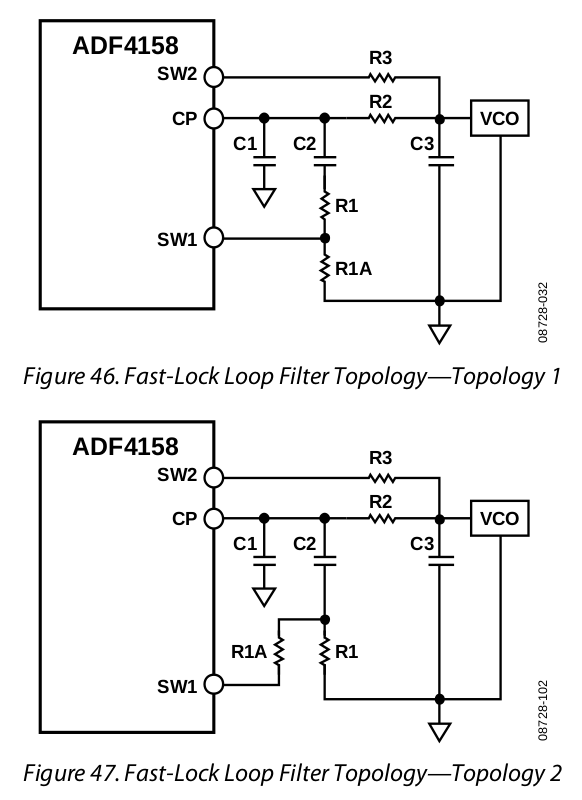
\includegraphics[width=0.5\textwidth]{data/adf4158-fast-lock.png}
        \caption{Fast lock topologies.}
        \label{fig:adf4158-fast-lock}
\end{figure}

\subsubsection{TLV2172 Operational Amplifier}
\label{sec:tlv2172-op-amp}

The \href{http://www.ti.com/lit/ds/symlink/tlv172.pdf}{TLV2172} op-amp is used to produce a gain of
2 to match the CP output of the ADF4158 to the VTUNE input of the VCO. This is necessary since the
charge pump supports a tune voltage of up to 5.5V but the VCO has a tune range of 0V to 10V. A
non-inverting amplifier configuration is used to produce the necessary gain.

\subsection{HMC431LP4RF VCO}
\label{sec:hmc431lp4rf}

The
\href{http://www.analog.com/media/en/technical_documentation/data_sheets/hmc431.pdf}{HMC431LP4RF} is
a radio-frequency VCO.

\subsection{SE2567L Power Amplifier}
\label{sec:se2567l-power-amp}

\fxnote{I've changed this component with the SE5004L, which has higher power output. Everything
  from this section forward (within the TX section) will need to be changed.}

\subsection{Notes}
\label{sec:notes}

\subsubsection{MGA25203 $\rightarrow$ SE2567L Substitution}
\label{sec:mga25203-se2567l-sub}

The MGA-25203 power amplifier is now obsolete and there are no alternatives with an identical
interface. Therefore the design will need to be modified. The alternative I will use is the
\href{http://www.skyworksinc.com/uploads/documents/202425A.pdf}{SE2567L} which seems to be very
similar. There are a few small differences in addition to the pin differences: the original device
has a power output of 23dBm in contrast to the new device which has a power output of 21.5dBm when
VCC0,1=3.3V and VCC2,3=4.5V. I believe this is close enough to not create any issues, especially as
they are both quoted as having 30dB gain and are IEEE 802.11-compliant. Additionally, the original
device has a load current about twice that of the new device. Since the output powers are relatively
similar (and the overview of original design describes a 20dB gain), I don't believe this should be
an issue. The original chip contains BCTRL, BSW, and BSPLY that differ from the new chip. BCTRL
regulates the device current and is kept at a constant 2.8V. There is no analogous pin on the new
chip. BSW is an enable pin that turns on the device when set to 1.8V. When it is set to 0V, the
device is turned off. The original design uses a MOSFET transistor with a drain of 1.8V, source at
GND and gate controlled by the FPGA (when the gate is activated the BSW pin gets a voltage of 0V and
is disabled). The new chip contains an analogous pin, EN, which enables the power amplifier at the
input voltage level 3.3V and disables it at GND. So, to get analogous functionality, we should
connect the MOSFET drain to 3.3V instead of 1.8. Everything else should stay the same. BSPLY simply
received the input voltage of 3.3V. In the new chip, the pins that are different from the original
chip (and not already discussed) are VCC0-3 and DET. DET is a pin that outputs a voltage indicating
the power output. We should connect this to a DNP capacitor to GND to be able to detect the output
power of the amplifier with an ammeter. VCC0-1 should be connected to the 3.3V power supply. In
order to get the additional power output, we should connect VCC2-3 to a 4.5V power supply instead of
3.3V. Unfortunately, it isn't possible to simply repurpose the voltage divider to the BCTRL pin for
this since I do not know the internal impedance of the power amplifier IC and in general voltage
dividers are bad for supplying power. Additionally, the simple LP5907 voltage divider may not work
since it is only rated to 250mA of current, which doesn't leave much room above the 220mA expected
by the SE2567L. It seems to make the most sense to use the
\href{http://www.ti.com/lit/ds/symlink/tps7a91.pdf}{TPS7A91} which is rated to 1A. It has the
downside of requiring additional hardware which will need to be adjusted in the PCB accordingly. To
get the correct output voltage of 4.5V, we need to use Equation~\ref{eq:linear-reg-vout}. Since the
datasheet doesn't specify the resistors for a 4.5V output voltage this takes a bit of art to finding
the correct resistors. Ideally, we want resistors with a higher-value so that less power is
dissipated, and are commonly used to reduce cost and make them easier to replace if
necessary. Lastly, I'd like to keep the values in the ballpark of those specified in the datasheet
in case there are any other reasons I'm not thinking of. The values $R_2 = 1.47\si{k\Omega}$ and
$R_1 = 6.8\si{k\Omega}$ should work well.
%%% Local Variables:
%%% mode: latex
%%% TeX-master: "fmcw-radar"
%%% End:
